
\documentclass[12pt]{article}

\usepackage{sbc-template}

\usepackage{graphicx,url}

\usepackage[spanish]{babel}   
%\usepackage[latin1]{inputenc}  
\usepackage[utf8]{inputenc}  
\usepackage{verbatim}
\usepackage{listings}
\usepackage{xcolor}

\definecolor{verde}{rgb}{0,0.5,0}

\lstset{language=verilog,
                belowcaptionskip=1\baselineskip,
                breaklines=true,
                frame=false,
                xleftmargin=\parindent,
                showstringspaces=false,
                basicstyle=\footnotesize\ttfamily,
                keywordstyle=\bfseries\color{green!40!black},
                commentstyle=\itshape\color{purple!40!black},
                identifierstyle=\color{blue},
                stringstyle=\color{orange},
                numbers=left,
            }

\sloppy

\title{Implementación procesador MIPS\\ Facultad de Ciencias Exactas, Físicas y Naturales}

\author{Sardoy, Juan Manuel\inst{1}, Perez, Federico\inst{1}}


\address{Arquitectura de computadoras - FCEFyN\\
  Av. Velez Sarsfield 1600 --  Córdoba -- Argentina
  \email{jmsardoy@gmail.com, 0xfede07c8@gmail.com}
}

\begin{document} 

\maketitle

\begin{resumen}
  Este documento describe, de manera sintética, la implementación práctica del pipeline de un procesador que cumple con un subconjunto del set de instrucciones de la arquitectura MIPS IV de 32 bits. La implementación está basada en tecnologia FPGA, mediante el lenguaje Verilog. Este trabajo tiene como objeto el aprendizaje de los diferentes elementos más comunes de la arquitectura de computadoras, dado el encuadre académico del mismo.\\
  \textbf{Palabras clave}: MIPS, FPGA, pipeline.
\end{resumen}

\begin{abstract}
  This document describes, in a synthetic way, a practical implementation of the pipeline of a processor that is compliant with a subset of the MIPS IV 32bits architecture instruction set. This job has as objective, to build the basic knowledge of the computer's architecture cope of study. \\
  \textbf{Keywords}: MIPS, FPGA, pipeline.
\end{abstract}

\section{Introducción}

El trabajo, se encuentra dentro del marco de la asignatura de Arquitectura de Computadoras, de la FCEFyN de la Universidad Nacional de Córdoba, Argentina. Corresponde al trabajo final de la misma, el cual es requerimiento para su aprobación. 

Además de la implementación del procesador en sí, se mostrará como implementar los elementos auxiliares requeridos para su funcionamiento y programación, entre otras utilidades. El hardware utilizado será un dispositivo FPGA, de la marca Xilinx, al ser de esta empresa, con los que cuentan los autores del trabajo. 

Dentro de los elementos auxiliares, encontraremos el desarrollo de un sistema de comunicación directo con el procesador, mediante el protocolo UART. Además de éste, un mecanismo para cargar un programa en la RAM del procesador, como asi también funcionalidad de debugging (ejecución paso a paso y salída de valores de registros internos). También se mostrará la implementación y uso de software auxiliar para el ensamblado de los programas a ejecutar. 

Todo esto compondrá una suite básica de desarrollo de software de propósito general, cuyo entendimiento es el objetivo principal del trabajo y la materia.


\section{Referencias Teóricas} \label{sec:firstpage}

La técnica de \textit{pipeline} es la más común utilizada para la implementación de procesadores modernos de diferentes arquitecturas, dado el gran aumento de \textit{IPC} (instrucciones por ciclo) que éste provee.

MIPS son las siglas de /textit{Microprocessor without interlocked pipeline stages}. La primera versión de ésta arquitectura fue desarrollada en la Universidad de Stanford en 1981 por un equipo liderado por John. L. Hennesy. La idea era diseñar un procesador segmentado (idea ya muy conocida en esos momentos) pero sin interbloqueo entre capas. En esa época eran comunes los procesadores donde cada instrucción iba ejecutandose por cada capaz, mientras las otras permanecian inactivas. Esto llevaba a que el tiempo que demora en ejecutar la instrucción fuera el del tiempo en el que tarda en pasar por todas las capas, en contraste con el tiempo del camino crítico, como ocurre sin interbloqueo. 

Por esto mismo este trabajo tendrá como cuerpo principal, la aplicación de dicha técnica, para lo cual, a modo de guía, se seguirá la bibliografía de \textit{Patterson y Hennesy}, dado que expone y soluciona los problemas más comunes a la hora de la creación de un \textit{pipeline} genérico. Sin embargo, muchas partes de la implementación, quedan a cargo, y serán solucionadas por los autores, lo cual lo hace una implementación única de la arquitectura.

\section{Metodología}

Se utilizará una metodología incremental y modular para la implementación del pipeline y sus módulos complementarios. Esto mejora el entendimiento y fragmentación del problema, asi como también facilta su implementación, dado la complejidad del mismo. También esto es muy util a la hora del testing y el debugeado del sistema.

\section{Requerimientos del trabajo}\label{sec:consigna}

Los requerimientos provistos por la cátedra fueron los siguientes:

\begin{enumerate}
  \item Implementar el pipeline de un procesador MIPS, segmentado en las siguientes etapas:
  \begin{enumerate}
    \item IF (Instruction Fetch): Búsqueda de la instrucción en la memoria de programa.
    \item ID (Instruction Decode): Decodificación de la instrucción y lectura de registros.
    \item EX (Excecute): Ejecución de la instrucción propiamente dicha.
    \item MEM (Memory Access): Lectura o escritura desde/hacia la memoria de datos.
    \item WB (Write back): Escritura de resultados en los registros.
  \end{enumerate}
  \item En dicha arquitectura, implementar las siguientes instrucciones:
  \begin{enumerate}
    \item R-type (SLL, SRL, SRA, SLLV, SRLV, SRAV, ADDU, SUBU, AND, OR, XOR, NOR, SLT?
    \item I-Type (LB, LH, LW, LWU, LBU, LHU, SB, SH, SW, ADDI, ANDI, ORI, XORI, LUI, SLTI, BEQ, BNE, J, JAL)
    \item J-Type (JR, JALR)
  \end{enumerate}
  \item Debe poseer soporte (detección y manejo) de los siguientes tipos de riesgos:
  \begin{enumerate}
    \item Estructurales: Cuando dos o más instrucciones tratan de utilizar el mismo recurso en el mismo ciclo.
    \item Datos: Una etapa desea utilizar un dato antes de que esté listo. Se debe mantener el orden estricto de las lecturas y escrituras. 
    \item Control: Capacidad para tomar una decición sobre una condicion no evaluada.
  \end{enumerate}
\end{enumerate}

As Tabelas, Quadros e Figuras, assim como as legendas de Tabelas, Quadros e Figuras devem estar centralizadas se conterem apenas em uma linha (Figura~\ref{fig:figura1}), caso contrário devem estar tabuladas em 0.8cm em ambas as margens, como mostra a Figura~\ref{fig:figura2}. 

\begin{figure}[ht]
\centering
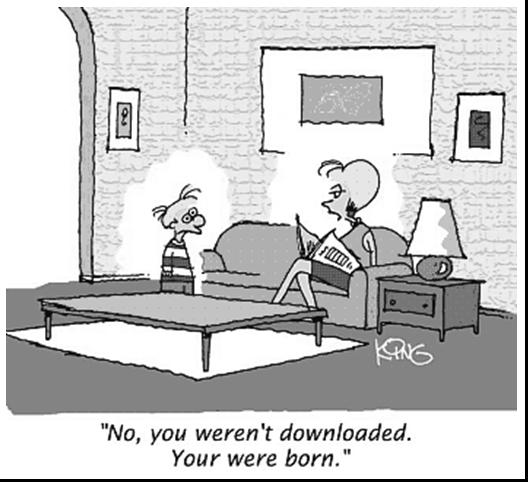
\includegraphics[width=.3\textwidth]{fig1.jpg}
\caption{Exemplo de figura}
\label{fig:figura1}
\end{figure}

As legendas devem ser escritas na fonte “Helvetica”, Tamanho 10pts, negrito, com espaço de 6pts antes e depois de cada legenda. Sempre que possível, procure colocar a figura delimitada por um quadro (Figura~\ref{fig:figura1} e Figura~\ref{fig:figura2})

\begin{figure}[!ht]
\centering
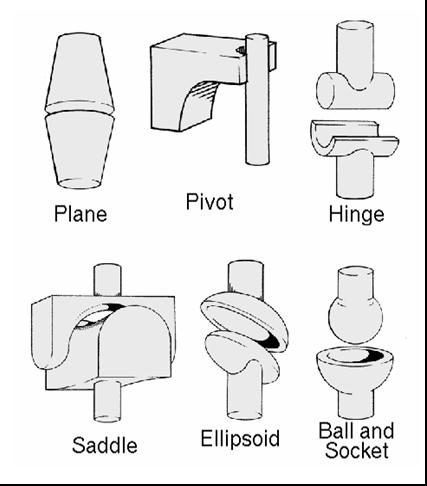
\includegraphics[width=.2\textwidth]{fig2.jpg}
\caption{Essa figura foi referenciada na Seção~\ref{sec:analisedosdados}.}
\caption{Fonte: SBC.}
\label{fig:figura2}
\end{figure}

Em tabelas, tente evitar o uso de fundos coloridos ou preenchidos, assim como linhas duplas na borda, ou linhas desnecessárias. Quando \cite{knuth:84} relatar dados empíricos, não faça uso de mais dígitos decimais do que o necessário. A legenda da tabela deve ser colocada antes da tabela (veja Tabela 1) e a fonte usada na legenda deve ser Helvetica, tamanho 10pts, negrito, com 6pts de espaço antes e depois de cada legenda.

\begin{table}[!ht]
\centering
\caption{Exemplo de tabela de 3 colunas e 2 linhas}
\label{tab:exTable1}
\smallskip
\begin{tabular}{l c c}
\hline
& Value 1 & Value 2\\[0.5ex]
\hline
&&\\[-2ex]
Case 1 & 1.0 $\pm$ 0.1 & 1.75$\times$10$^{-5}$ $\pm$ 5$\times$10$^{-7}$\\[0.5ex]
\hline
&&\\[-2ex]
Case 2 & 0.003(1) & 100.0\\[0.5ex]
\hline
\end{tabular}
\end{table}

\subsection{Código fonte}
A inserção de código fonte deve ser por meio

\begin{lstlisting}

int main(){
  int a,b,c;
  float x;
  printf("informe o tamanho do lado do quadrado");
  scanf("%d", &a);
  printf("A area do quadrado %d", b=area(a));
  printf("Duas vezes o valor do lado do quadrado %d", c=aumenta(a));

\end{lstlisting}



\section{Considerações Finais}

Referências bibliográficas devem ser utilizadas dentro de um estilo uniforme e não ambíguo. A SBC sugere os seguintes formatos para referências: \cite{knuth:84}, \cite{boulic:91}, e \cite{smith:99}.

\bibliographystyle{sbc}
\bibliography{sbc-template}

\end{document}
